% Capitolo 5: Pattern Matching - Fondamenti

\chapter{Pattern Matching: Problemi e Soluzioni}
\label{cap:pattern_matching}

\section{Introduzione}

Il pattern matching è l'operazione fondamentale nei sistemi a produzione: determinare quali regole sono applicabili dato un certo stato della working memory. L'efficienza di questa operazione determina le prestazioni dell'intero sistema.

\subsection{Il Problema Centrale}

Dato:
\begin{itemize}
\item Un insieme di regole $R = \{r_1, r_2, \ldots, r_n\}$
\item Una working memory $WM = \{f_1, f_2, \ldots, f_m\}$ di fatti
\end{itemize}

\textbf{Obiettivo}: Trovare tutte le \textit{istanziazioni} (binding di variabili) che soddisfano le condizioni LHS di ogni regola.

\begin{definizione}[Istanziazione]
Un'istanziazione $\iota$ di una regola $r$ è un assegnamento di valori alle variabili di $r$ tale che tutti i pattern della LHS matchano fatti in $WM$.
\end{definizione}

\section{Approccio Naïve}

\subsection{Algoritmo di Base}

\begin{algorithm}
\caption{Pattern Matching Naïve}
\begin{algorithmic}[1]
\Require Regole $R$, Working Memory $WM$
\Ensure Conflict Set $CS$
\Function{NaiveMatch}{$R, WM$}
  \State $CS \gets \emptyset$
  \For{each rule $r \in R$}
    \For{each combinazione di fatti $(f_1, \ldots, f_k) \in WM^k$}
      \If{$(f_1, \ldots, f_k)$ soddisfa LHS di $r$}
        \State $CS \gets CS \cup \{(r, f_1, \ldots, f_k)\}$
      \EndIf
    \EndFor
  \EndFor
  \State \Return $CS$
\EndFunction
\end{algorithmic}
\end{algorithm}

\subsection{Complessità}

Per ogni regola con $k$ condizioni e $m$ fatti in WM:
\begin{equation}
O(m^k)
\end{equation}

Con $n$ regole:
\begin{equation}
O(n \cdot m^k)
\end{equation}

\begin{warningbox}[Esplosione Combinatoria]
Con 100 regole, 1000 fatti, e media di 3 condizioni per regola:
\begin{equation}
100 \cdot 1000^3 = 10^{11} \text{ operazioni per ciclo}
\end{equation}
Assolutamente impraticabile!
\end{warningbox}

\section{Principio di Temporalità}

\subsection{Osservazione Chiave}

Tra un ciclo recognize-act e il successivo:
\begin{itemize}
\item La maggior parte dei fatti \textbf{non cambia}
\item Solo pochi fatti vengono aggiunti/rimossi
\item La maggior parte dei match \textbf{rimane valida}
\end{itemize}

\begin{definizione}[Principio di Temporalità]
In un sistema a produzione, tra cicli consecutivi:
\begin{equation}
|WM_{t+1} \triangle WM_t| \ll |WM_t|
\end{equation}
dove $\triangle$ indica la differenza simmetrica.
\end{definizione}

\textbf{Implicazione}: Ricalcolare tutto da zero spreca lavoro. Dobbiamo \textit{incrementare} il risultato.

\subsection{Approccio Incrementale}

Idea: Memorizzare i match parziali e aggiornarli solo quando necessario.

\begin{infobox}[State Saving]
\begin{itemize}
\item \textbf{Salvare}: Match intermedi tra cicli
\item \textbf{Riutilizzare}: Risultati precedenti
\item \textbf{Aggiornare}: Solo quando fatti cambiano
\item \textbf{Guadagno}: Evitare ricalcoli ridondanti
\end{itemize}
\end{infobox}

\section{Discriminazione}

\subsection{Pattern Simili}

Molte regole condividono parti delle condizioni:

\begin{lstlisting}[language=CLIPS]
;; Regola 1
(defrule r1
  (persona (eta ?e&:(> ?e 18)))
  =>
  ...)

;; Regola 2  
(defrule r2
  (persona (eta ?e&:(> ?e 18)))
  (studente (id ?id))
  =>
  ...)

;; Regola 3
(defrule r3
  (persona (eta ?e&:(> ?e 65)))
  =>
  ...)
\end{lstlisting}

Tutte e tre testano \texttt{persona} con constraint sull'età.

\subsection{Condivisione dei Test}

\begin{definizione}[Discriminazione]
La discriminazione è il processo di \textit{condividere} test comuni tra regole diverse per evitare duplicazione di lavoro.
\end{definizione}

\textbf{Beneficio}: Un test effettuato una volta serve multiple regole.

\begin{figure}[h]
\centering
\begin{tikzpicture}[
  node distance=2cm,
  test/.style={rectangle, draw, minimum width=2cm, minimum height=0.8cm},
  result/.style={ellipse, draw, minimum width=1.5cm}
]
  \node[test] (root) {tipo = persona};
  \node[test, below left of=root] (left) {età > 18};
  \node[test, below right of=root] (right) {età > 65};
  \node[result, below of=left] (r1r2) {R1, R2};
  \node[result, below of=right] (r3) {R3};
  
  \draw[->] (root) -- (left);
  \draw[->] (root) -- (right);
  \draw[->] (left) -- (r1r2);
  \draw[->] (right) -- (r3);
\end{tikzpicture}
\caption{Albero di discriminazione per test comuni}
\label{fig:discriminazione}
\end{figure}

\section{Confronto tra Approcci}

\subsection{Tabella Comparativa}

\begin{table}[h]
\centering
\begin{tabular}{@{}lccc@{}}
\toprule
\textbf{Metodo} & \textbf{Spazio} & \textbf{Tempo/ciclo} & \textbf{Incrementale} \\
\midrule
Naïve & $O(1)$ & $O(n \cdot m^k)$ & No \\
Linear & $O(n)$ & $O(n \cdot m)$ & Parziale \\
RETE & $O(n \cdot m^k)$ & $O(m)$ & Sì \\
\bottomrule
\end{tabular}
\caption{Confronto algoritmi di pattern matching}
\label{tab:confronto_matching}
\end{table}

\subsection{Trade-off Spazio-Tempo}

RETE rappresenta il classico trade-off:
\begin{itemize}
\item \textbf{Più spazio}: Memorizza match parziali
\item \textbf{Meno tempo}: Aggiornamenti incrementali
\end{itemize}

\textbf{Quando conviene}:
\begin{equation}
\text{Costo}(\text{spazio extra}) < \text{Beneficio}(\text{tempo risparmiato})
\end{equation}

Per sistemi con:
\begin{itemize}
\item Molti cicli recognize-act
\item WM moderatamente grande ($m \gg 10$)
\item Cambiamenti piccoli tra cicli
\end{itemize}

RETE è quasi sempre vantaggioso.

\section{Join di Pattern}

\subsection{Il Problema del Join}

Quando due pattern condividono variabili, dobbiamo verificare consistenza:

\begin{lstlisting}[language=CLIPS]
(defrule stesso-reparto
  (impiegato (id ?id1) (reparto ?r))
  (impiegato (id ?id2&~?id1) (reparto ?r))  ; Stessa variabile ?r!
  =>
  ...)
\end{lstlisting}

\subsection{Join in Database}

Analogo al join relazionale:

\begin{equation}
R_1 \bowtie_{\theta} R_2 = \{(t_1, t_2) \mid t_1 \in R_1, t_2 \in R_2, \theta(t_1, t_2)\}
\end{equation}

dove $\theta$ è una condizione di join.

\textbf{Tecniche classiche}:
\begin{itemize}
\item \textbf{Nested loop join}: $O(|R_1| \cdot |R_2|)$
\item \textbf{Hash join}: $O(|R_1| + |R_2|)$ con preprocessing
\item \textbf{Sort-merge join}: $O(|R_1| \log |R_1| + |R_2| \log |R_2|)$
\end{itemize}

\subsection{Join in RETE}

RETE usa hash join incrementale:
\begin{enumerate}
\item Memorizza match parziali in hash table
\item Nuovo fatto $\rightarrow$ lookup nella hash table
\item Crea nuovi match combinando
\end{enumerate}

\textbf{Complessità amortizzata}: $O(1)$ per inserimento.

\section{Tipi di Pattern}

\subsection{Pattern Intra-elemento}

Test su un singolo fatto:

\begin{lstlisting}[language=CLIPS]
(persona (eta ?e&:(> ?e 18)&:(< ?e 65)))
\end{lstlisting}

\textbf{Complessità}: $O(m)$ - scansione lineare dei fatti.

\subsection{Pattern Inter-elemento}

Test che coinvolgono multiple condizioni:

\begin{lstlisting}[language=CLIPS]
(impiegato (id ?id) (stipendio ?s1))
(bonus (impiegato ?id) (importo ?b))
(test (> ?b (* 0.2 ?s1)))  ; Bonus > 20% stipendio
\end{lstlisting}

\textbf{Complessità}: Dipende dal numero di combinazioni.

\subsection{Pattern Negativi}

Negazione (assenza di match):

\begin{lstlisting}[language=CLIPS]
(not (ordine (cliente ?id)))
\end{lstlisting}

\textbf{Semantica}: Vero se \textit{non esiste} un match.

\textbf{Sfida}: Quando invalidare? Quando un fatto che match appare.

\section{Gestione della Negazione}

\subsection{Negation as Failure (NAF)}

\begin{definizione}[NAF]
Un pattern negato $(not~\varphi)$ è soddisfatto se non esiste binding che soddisfa $\varphi$.
\end{definizione}

\textbf{Problema}: Non monotonia.

\begin{esempio}[Non Monotonia della Negazione]
\begin{enumerate}
\item Stato iniziale: WM = $\{(persona~\text{"Mario"})\}$
\item Regola: \texttt{(persona ?x) (not (ordine ?x)) => ...}
\item Match esiste: Mario non ha ordini
\item Aggiungi: \texttt{(ordine "Mario")}
\item Match \textbf{scompare}!
\end{enumerate}
\end{esempio}

\subsection{Implementazione in RETE}

RETE gestisce la negazione con \textit{nodi beta negativi}:

\begin{itemize}
\item Mantengono count di match nel pattern negato
\item Count = 0 $\Rightarrow$ pattern negato soddisfatto
\item Aggiornano count incrementalmente
\end{itemize}

\section{Variabili Multifield}

\subsection{Challenge}

Le variabili multifield matchano zero o più valori:

\begin{lstlisting}[language=CLIPS]
(lista $?inizio 10 $?fine)
\end{lstlisting}

Match possibili per \texttt{(lista 1 2 10 3 4)}:
\begin{itemize}
\item $\texttt{\$?inizio} = [1,2]$, $\texttt{\$?fine} = [3,4]$
\item $\texttt{\$?inizio} = [1,2,10]$, $\texttt{\$?fine} = []$ (no, 10 deve essere letterale)
\end{itemize}

\subsection{Complessità}

Con $n$ multifield variables e fatto di lunghezza $k$:
\begin{equation}
O\left(\binom{k}{n}\right) \text{ possibili partizioni}
\end{equation}

\textbf{Esplosione combinatoria}: Evitare multifield non vincolate.

\begin{warningbox}[Best Practice]
Specificare sempre constraint o ancoraggi per multifield:
\begin{lstlisting}[language=CLIPS]
;; Meglio
(lista primo $?resto&:(> (length$ ?resto) 0))

;; Peggio (troppe possibilita)
(lista $?a $?b $?c)
\end{lstlisting}
\end{warningbox}

\section{Ordinamento dei Pattern}

\subsection{Selettività}

\begin{definizione}[Selettività]
La selettività di un pattern è la frazione di fatti in WM che lo soddisfano:
\begin{equation}
\text{sel}(p) = \frac{|\{f \in WM \mid f \text{ matches } p\}|}{|WM|}
\end{equation}
\end{definizione}

\subsection{Ordinamento Ottimale}

\textbf{Principio}: Valutare prima i pattern più selettivi.

\begin{teorema}[Ordinamento Ottimale]
Data una regola con pattern $p_1, \ldots, p_n$, l'ordinamento che minimizza il costo atteso è quello per selettività crescente:
\begin{equation}
\text{sel}(p_1) \leq \text{sel}(p_2) \leq \ldots \leq \text{sel}(p_n)
\end{equation}
\end{teorema}

\textbf{Intuizione}: Eliminare candidati presto riduce il lavoro successivo.

\subsection{Stima della Selettività}

\textbf{Tecniche}:
\begin{itemize}
\item \textbf{Statistiche}: Raccogliere durante esecuzione
\item \textbf{Euristica}: Pattern con più constraint $\Rightarrow$ più selettivo
\item \textbf{Profiling}: Analizzare run precedenti
\end{itemize}

\section{Indici e Strutture Dati}

\subsection{Hash Index}

Per pattern del tipo \texttt{(persona (id 123))}:

\begin{itemize}
\item Indicizzare fatti per tipo e slot
\item Hash su valore per accesso $O(1)$
\end{itemize}

\subsection{Trie per Pattern}

Per pattern complessi, trie discrimina su prefissi comuni:

\begin{figure}[h]
\centering
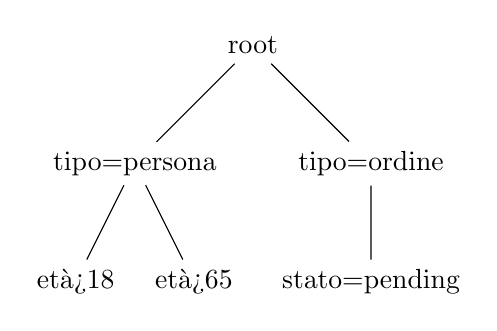
\begin{tikzpicture}[
  level distance=1.5cm,
  level 1/.style={sibling distance=3cm},
  level 2/.style={sibling distance=1.5cm}
]
  \node {root}
    child {node {tipo=persona}
      child {node {età>18}}
      child {node {età>65}}
    }
    child {node {tipo=ordine}
      child {node {stato=pending}}
    };
\end{tikzpicture}
\caption{Trie per discriminazione pattern}
\end{figure}

\section{Confronto con Altri Paradigmi}

\subsection{Query in Database}

\textbf{Somiglianze}:
\begin{itemize}
\item Pattern = query SQL
\item Working Memory = tabelle
\item Join di pattern = join relazionali
\end{itemize}

\textbf{Differenze}:
\begin{itemize}
\item DB: query singola su snapshot
\item CLIPS: query continue su stream di aggiornamenti
\item RETE: "standing queries" materializzate
\end{itemize}

\subsection{Pattern Matching Funzionale}

In linguaggi come Haskell/ML:

\begin{verbatim}
fib 0 = 0
fib 1 = 1  
fib n = fib (n-1) + fib (n-2)
\end{verbatim}

\textbf{Differenze}:
\begin{itemize}
\item Matching su struttura dati (non DB)
\item Sequenziale (non parallelo)
\item Deterministico (primo match vince)
\end{itemize}

\section{Metriche di Performance}

\subsection{Metriche Chiave}

\begin{table}[h]
\centering
\begin{tabular}{@{}ll@{}}
\toprule
\textbf{Metrica} & \textbf{Descrizione} \\
\midrule
Tempo per ciclo & Latenza recognize-act \\
Throughput & Cicli/secondo \\
Utilizzo memoria & Spazio per match parziali \\
Hit rate & Frazione match riutilizzati \\
Conflict set size & Numero attivazioni per ciclo \\
\bottomrule
\end{tabular}
\caption{Metriche di performance pattern matching}
\end{table}

\subsection{Profiling}

Strumenti per analizzare bottleneck:
\begin{itemize}
\item Tempo per nodo RETE
\item Distribuzione di firing
\item Crescita memoria nel tempo
\item Pattern più/meno selettivi
\end{itemize}

\section{Limiti e Problemi Aperti}

\subsection{Worst Case}

Anche RETE ha worst case $O(n \cdot m^k)$ quando:
\begin{itemize}
\item Tutti i fatti cambiano ogni ciclo
\item Pattern molto generici (bassa selettività)
\item Join con Cartesian product
\end{itemize}

\subsection{Problemi Aperti}

\begin{itemize}
\item \textbf{Adaptive indexing}: Riottimizzare indici dinamicamente
\item \textbf{Parallel matching}: RETE su GPU/multicore
\item \textbf{Distributed matching}: RETE su cluster
\item \textbf{Approximate matching}: Tolleranza a errori/rumore
\item \textbf{Learning}: Apprendere ordinamento pattern ottimale
\end{itemize}

\section{Conclusioni del Capitolo}

\subsection{Punti Chiave}

\begin{enumerate}
\item Pattern matching naïve è impraticabile per sistemi reali
\item Il \textbf{principio di temporalità} giustifica approcci incrementali
\item La \textbf{discriminazione} permette condivisione di lavoro
\item Join e negazione richiedono tecniche speciali
\item Trade-off spazio-tempo favorisce RETE in pratica
\end{enumerate}

\subsection{Prossimi Capitoli}

\begin{itemize}
\item Capitolo~\ref{cap:rete_introduzione}: Introduzione dettagliata a RETE
\item Capitolo~\ref{cap:rete_alpha}: Rete Alpha (discriminazione)
\item Capitolo~\ref{cap:rete_beta}: Rete Beta (join e negazione)
\item Capitolo~\ref{cap:rete_complessita}: Analisi di complessità formale
\item Capitolo~\ref{cap:rete_ottimizzazioni}: Ottimizzazioni e varianti
\end{itemize}

\subsection{Letture Consigliate}

\begin{itemize}
\item Forgy, C. (1982). "Rete: A Fast Algorithm for the Many Pattern/Many Object Pattern Match Problem"
\item Forgy, C. (1984). "The Rete Algorithm Detailed"
\item Giarratano \& Riley (2004). "Expert Systems" - Cap. 8
\item Brownston et al. (1985). "Programming Expert Systems in OPS5"
\item Doorenbos, R. (1995). "Production Matching for Large Learning Systems" (RETE/UL)
\end{itemize}
